\chapter{Introduction}
\label{chp:introduction}
Tribler is a peer-to-peer BitTorrent client that attempts to fully decentralize downloading, uploading and streaming of content.

Tribler focusses on the goals:
\begin{itemize}
    \item Allow for secure and private communication and sharing of data.
    \item Enforce user contribution in the network
    \item Make it impossible to shut Tribler down, unless the Internet itself as a whole gets taken down.
\end{itemize}

A fully decentralized ecosystem i.e. no central components present, is Tribler's approach to achieve these goals.
Tribler has been designed and build with this focus~\cite{Pouwelse-tribler,Bakker-tribler}.
A distributed network requires both the presence and collaboration of participants, called peers, to be able to achieve this.

This thesis was conducted to improve the connectability and overall performance of Tribler, by identifying and removing bottlenecks present in the system.

\begin{figure}
	\centerline{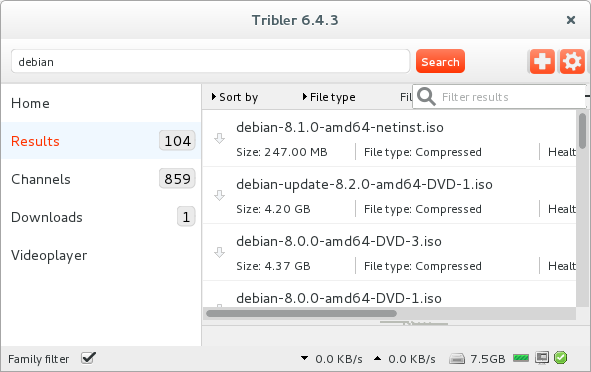
\includegraphics[scale=0.6]{introduction/figs/tribler-screenshot.png}}
	\caption{Screenshot of Tribler v6.4.3.}
	\label{fig:tribler-screenshot}
\end{figure}

\section{BitTorrent protocol}
When sharing files by using the BitTorrent protocol, a peer that uploads parts of a file to another peer, is called a seeder.
A peer that is downloading a file of a seeder is called a leecher.
Any peer can be both a seeder and leecher at the same time, and join the network at any given time.

The ratio between the total data downloaded and uploaded is called the seeding ratio~\cite{Cohen-bittorrent}.
The seeding ratio can be seen as an indication of the level of collaboration i.e. giving back resources to the network.

Seeding can be seen as an interaction between peers, where the seeder aids the leeching peer.
By utilizing the seeders upload bandwith, the leeching peer can use his download bandwidth to download a file.
While there is a clear incentive for the leecher by downloading the desired file, there is none for the seeder.
Especially since the leecher has a little chance of becoming also be a seeder for the original seeder~\cite{Lai-Incentives}.

Having peers actively and persistently contribute to the network will increase the network's health which in turn provides several benefits for all peers.
A more healthy network results in a higher availability of seeders and results in high download speeds.
It has been shown that private communities where the seeding ratio is high, provides better download conditions \cite{meulpolder-privatecommunities}.
In these private communities, trackers i.e. central components introduce peers to each other using the Tit-for_tat approach \cite{cohen-titfortat}.
The Tit-for-Tat approach is aiding peers who have aided you in the past, 

The absence of trackers, which is often the case in public networks, results in free-riding \cite{Adar-Freeriding}.
A free-riding peer does not or gives little back to the network while receiving all benefits i.e. download without any restriction.
BitTorrent applies the Tit-for_tat strategy to combat this problem, yet it has been shown that this approach is not effective \cite{Pouwelse-tribler}.
The Tit-for-Tat strategy is to only provide help to peers to peers that return this help.
% TODO explain the optimistic chocking approach

\section{Tribler}

Tribler wants to achieve a high global seeding ratio by making it beneficial to have such a ratio.
Nodes can award each other with higher cooperation if a node has a reputation of being cooperative,
while malicious nodes are prevented from tampering and freeriding.
Within Tribler anonymous connections have been implemented recently using onion routing~\cite{Plak-anonymous,ruigrok-anonymous,tanaskoski-anonymous}.
This feature allows downloaders to become indistinguishable from other users in the network save guarding their privacy.
Every data packet has to be forwarded
by a number of intermediate hops between the downloader and seeder~\cite{Plak-anonymous,tanaskoski-anonymous}.
The total cost of bandwidth per file is increased,
because it has to be forwarded by multiple nodes.
but also the number of nodes helping a single node downloading a file increases.
The increase in nodes working together increases the necessity of an incentive system to reward collaboration.

Dispersy is middleware for data dissemination in a network.
Dispersy is used heavily within Tribler and is maintained by the Tribler organisation.
Our work is build upon Dispersy.
Dispersy is used to exchange data between two specific nodes~\cite{zeilemaker-dispersy}.
Functionality was added to Dispersy during the thesis.
The additions are described in chapter \ref{chapt:design}.

\section{Document structure}
Chapter \ref{chp:introduction} provides information on Tribler.
Chapter \ref{chp:problem-description} presents an overview of some of the problems Tribler is currently facing.
